\section{Eksperymenty}
W naszym projekcie przeprowadziliśmy walidacji krzyżowej dla parametru k równego 10 dla drzewa utworzonego przez algorytm ID3 oraz dla drzewa utworzonego prze C4.5.

\subsection{Wyniki}



\begin{table}[H]
    \centering
    \begin{tabular}{|c|c|}
    \hline
    Algorytm                & Dopasowanie         \\ \hline
    ID3                     & 81,5\%              \\ \hline
    C4.5                    & 81,4\%              \\ \hline
    \end{tabular}
    \caption{Wyniki walidacji krzyżowej dla akceptorów}
    \label{tab:crossing}
\end{table}

\begin{table}[H]
    \centering
    \begin{tabular}{|c|c|}
    \hline
    Algorytm                & Dopasowanie         \\ \hline
    ID3                     & 83,2\%              \\ \hline
    C4.5                    & 81,7\%              \\ \hline
    \end{tabular}
    \caption{Wyniki walidacji krzyżowej dla donorów}
    \label{tab:crossing}
\end{table}

Z wyników walidacji...

\begin{figure}[H]
    \centering 
    \begin{subfigure}[b]{0.49\linewidth}
        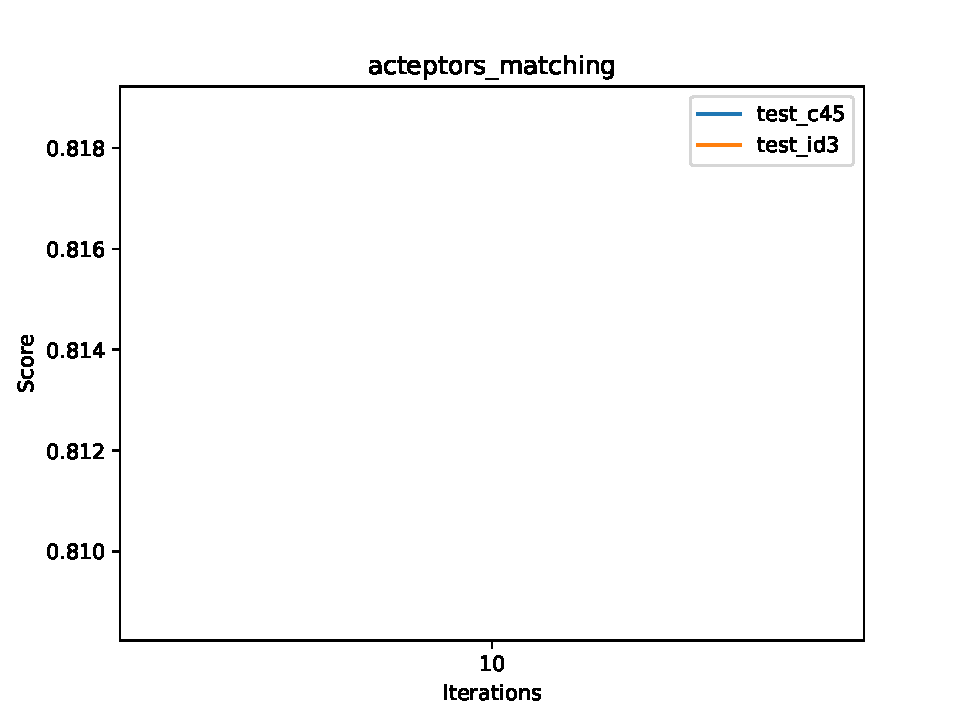
\includegraphics[width=\linewidth]{img/acteptors_matching.pdf}
        \caption{$\mu$ = 2}
    \end{subfigure}
    \begin{subfigure}[b]{0.49\linewidth}
        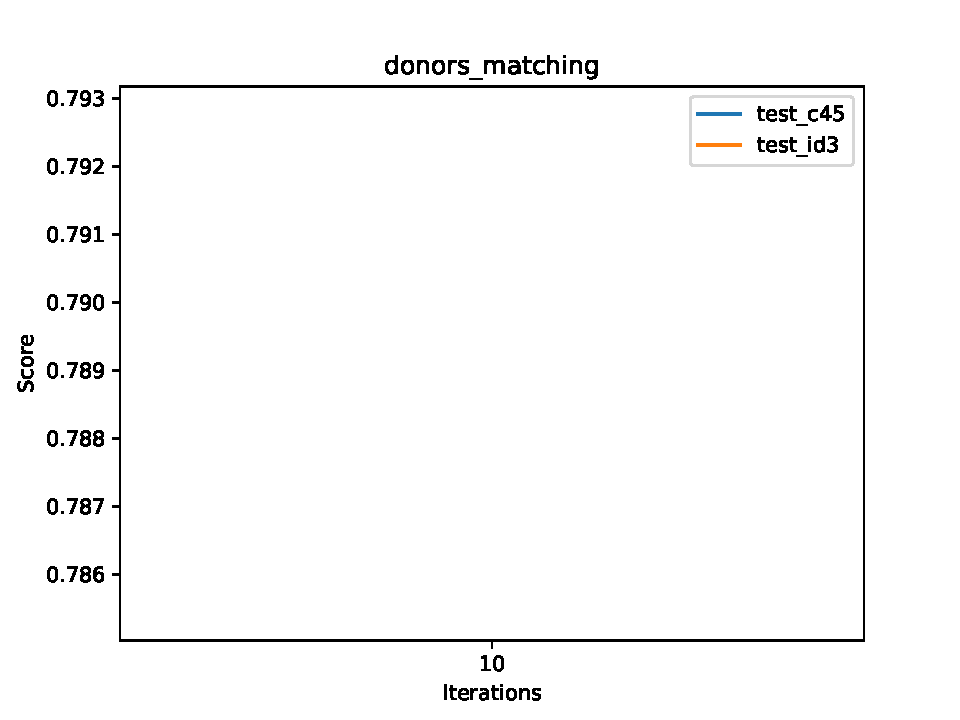
\includegraphics[width=\linewidth]{img/donors_matching.pdf}
        \caption{$\mu$ = 10}
    \end{subfigure}
    \caption{Akceptory i donory}
    \label{fig:picking}
\end{figure}

